\documentclass[svgnames,10pt]{standalone}
\usepackage[utf8]{inputenc}
\usepackage[T1]{fontenc}
\usepackage{csquotes}
\usepackage[english]{babel}
\usepackage{xcolor}
\usepackage{charter}
\usepackage{amsmath}
\usepackage{amssymb}
\usepackage[np,autolanguage]{numprint}
\newcommand{\outqt}[1]{{\textcolor{DarkOrange}{#1}}}
\newcommand{\inqt}[1]{{\textcolor{Blue}{#1}}}
\usepackage{tikz}
\usetikzlibrary{arrows,automata,calc}
\usetikzlibrary{arrows.meta}
\usetikzlibrary{decorations.pathreplacing}
\usetikzlibrary{backgrounds,shapes}
\tikzset{%
  show curve controls/.style={
    postaction={
      decoration={
        show path construction,
        curveto code={
          \draw [blue] 
            (\tikzinputsegmentfirst) -- (\tikzinputsegmentsupporta)
            (\tikzinputsegmentlast) -- (\tikzinputsegmentsupportb);
          \fill [red, opacity=0.5] 
            (\tikzinputsegmentsupporta) circle [radius=.25ex]
            (\tikzinputsegmentsupportb) circle [radius=.25ex];
        }
      },
      decorate
}}}
\tikzstyle{vertex}=[draw,circle,black,inner sep=2pt]
\tikzstyle{edge}=[line width=1.3pt,color=Black]
\tikzstyle{rare}=[fill=black,text=white]
\tikzstyle{medium}=[fill=black!15!white]


\tikzstyle{legend}=[inner sep=0pt,black,font=\small]
\tikzstyle{pose}=[line width=2.0pt,solid,black]
\tikzstyle{nege}=[line width=2.0pt,dashed,black]
\tikzstyle{c1}=[fill=DodgerBlue]
\tikzstyle{c2}=[fill=Orange]
\tikzstyle{c3}=[fill=SpringGreen]
\begin{document}
  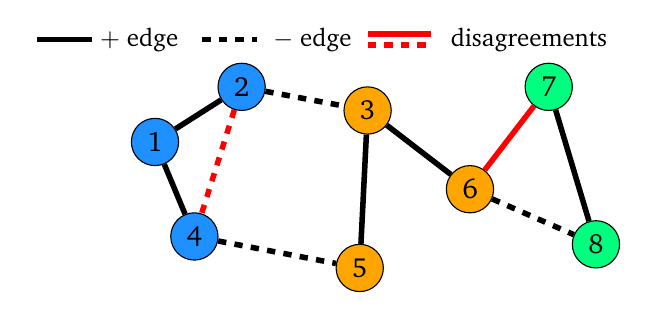
\begin{tikzpicture}[auto, vertex/.append style={minimum width=6mm}]
    \foreach \place/\name in { {(-0.5,2.6)/1}, {(0.6,3.3)/2}, {(0,1.4)/4}}
      \node[vertex,c1] (\name) at \place {\name};
    \foreach \place/\name in {{(2.2,3)/3}, {(2.1,1)/5}, {(3.5,2)/6}}
      \node[vertex,c2] (\name) at \place {\name};
    \foreach \place/\name in  {{(4.5,3.3)/7}, {(5.1,1.3)/8}}
      \node[vertex,c3] (\name) at \place {\name};
    \foreach \source/\dest in {1/2, 1/4, 3/5, 3/6, 7/8}
      \draw[pose] (\source) edge  (\dest);
    \foreach \source/\dest in {2/3,4/5,6/8}
      \draw[nege] (\source) edge  (\dest);

    \draw[pose] (-2,3.9) edge (-1.3,3.9) node (poslegend) {};
    \node[legend] at (-0.7,3.9) {$+$ edge};
    \draw[nege] (0.1,3.9) edge (0.8,3.9) node (neglegend) {};
    \node[legend] at (1.5,3.9) {$-$ edge};
    \draw[pose,red] (2.2,3.97) edge (3,3.97);
    \draw[nege,red] (2.2,3.83) edge (3,3.83);
    \node[legend] at (4.25,3.9) {disagreements};

    \draw[pose,red] (6) edge  (7);
    \draw[nege,red] (2) edge  (4);
  \end{tikzpicture}
\end{document}
